\documentclass[twoside]{ctexbook}
% 大32开,148×210(mm),4.625x6.5625英寸
\usepackage[smartEllipses]{markdown}
\usepackage{pdfpages}
\usepackage{xcolor}

\definecolor{crany}{HTML}{304FFE}
\usepackage{hyperref}
\hypersetup{%
    pdfborder = {0 0 0},
    colorlinks,
    citecolor=red,
    filecolor=Darkgreen,
    linkcolor=crany,
    urlcolor=cyan!50!black!90
}
\usepackage{geometry}
\geometry{
	paperwidth=148mm, 
	paperheight=210mm,
	width=100mm,%width=104mm,
%	height=149mm,
	headsep=13mm,
	headheight=3mm,
	footskip=14mm,
	right=23mm,%right=21mm,
	top=32mm
  }

\usepackage{fancyhdr}
\pagestyle{fancy}
\fancyhf{}
\renewcommand{\headrulewidth}{0pt}
 \fancyhead[EL]{\zihao{-5}\color{crany}|~闲言碎语}
 \fancyhead[OR]{\zihao{-5}\color{crany}\leftmark~|}
 \fancyhead[OL,ER]{}
 \fancyhead[C]{}
 \fancyfoot[C]{\zihao{-5}\color{crany}\thepage}


\fancypagestyle{plain}{
\fancyhead{}
\fancyfoot[C]{\zihao{-5}\color{crany}\thepage}
} 


\ctexset{
chapter/name={},
chapter/numbering=false,
chapter/format +=  \color{crany},
chapter/beforeskip=10pt,
chapter/afterskip=50pt,
section/numbering=false,
section/format +=  \color{crany}\zihao{5}\raggedright,
section/beforeskip=1.2ex,
section/afterskip=0.2ex,
section/afterindent=false,
space=true,
}
\linespread{1.5}

\usepackage{layout}
\makeatletter
\renewcommand*{\lay@value}[2]{%
  \strip@pt\dimexpr0.351459\dimexpr\csname#2\endcsname\relax\relax mm%
}
\makeatother

\begin{document}
%\layout % \\输出页面边界信息
\zihao{5}

% 封面信息
% \thispagestyle{empty}

% 
\includepdf{doc/hardcover.pdf}
% \thispagestyle{empty}
% \newpage
% \ % The empty page
% \thispagestyle{empty}
% \newpage
\thispagestyle{empty}
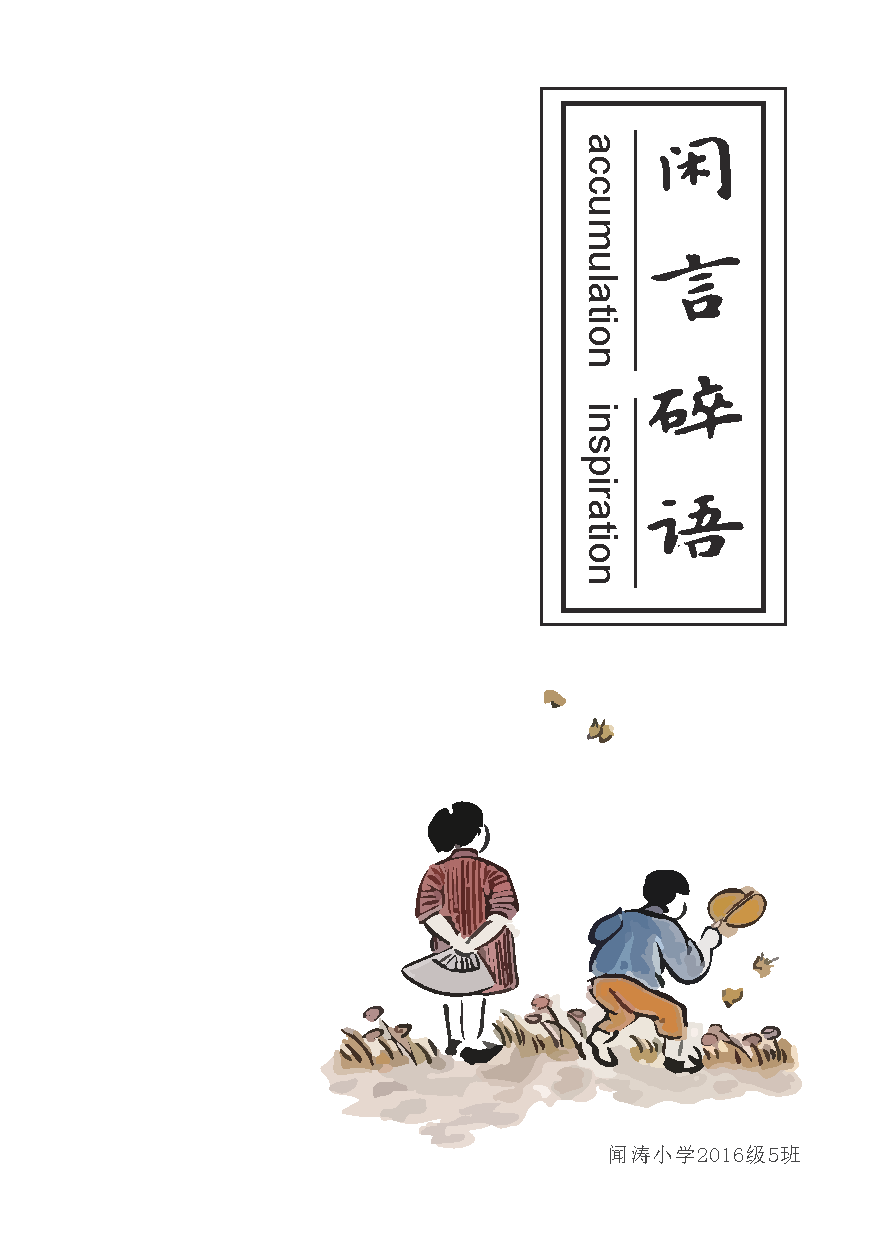
\includepdf{doc/cover.pdf}

\clearpage

\thispagestyle{empty}
\vspace*{\fill}

\begin{flushleft}
  \begingroup

  主\hspace*{2\ccwd}编:詹慧丽\\
  装帧设计:杨建林\\
  \endgroup
\end{flushleft}
\vspace{3em}
\begin{flushleft}

  \begingroup

  书\hspace*{2\ccwd}名:闲言碎语\\
  版\hspace*{2\ccwd}次:2022年5月 第一版\\
  开\hspace*{2\ccwd}本:889mm x 1194mm  1/32\\
  字\hspace*{2\ccwd}数:70 千字\\
  印\hspace*{2\ccwd}数:50 册\\
  定\hspace*{2\ccwd}价:38.00 元\\
  \vspace{2em}
  印刷、装订质量问题,出版社负责调换。
  \endgroup
\end{flushleft}

\zihao {5}
\clearpage

\thispagestyle{empty}

\vspace*{3em}
\hspace{3em}\songti{献给,起点的回忆}
\newpage
\thispagestyle{empty}
\
\newpage
\setcounter{page}{1}
\heiti{\tableofcontents}
\thispagestyle{empty}

\songti
\mainmatter
\hypersetup{pageanchor=true}


\chapter*{《序》}
\addcontentsline{toc}{chapter}{《序》}
\markboth{《序》}{}
闲言碎语是一个非常有意思的活动,题材不限,内容不限。在这里你可以天马行空肆意发挥,可以细致入微洞察秋毫。另一方面,活动是3、4个同学共写一本日记本,所以同学间可以相互借鉴,相互督促。可以参考小组其他同学是怎么写的,写的什么题材。

我们在班级公众号会定期整理发布闲言碎语每日之最,以供大家鉴赏、鞭策。同学们写的文章生动有趣,仿佛把我们也带回了快乐的童年。

但是,并不代表没被评为每日之最的文章就不好。也许写作无关文笔好坏,能打动自己的文字,一定会打动世界某个角落的某个人。用文字记录下所见所思,照见自己内心,坚持下去。

文字是生命的延续。人生不过百年,而文字却可以长久的流传下去。老子道德经五千言,几千年来流淌在华夏儿女的血脉中。司马迁忍辱负重创作鸿篇巨著《史记》,使得我们能了解到中华文明的渊源。

所以,请拿起手中的笔,坚持写下去。以前一位朋友引用某位名人的话告诉我:如果你坚持不下去,那么就坚持下去吧。我修改下,送给各位同学:如果你不知道写什么,那就写点什么吧。

\markdownInput{doc/1.md}
\markdownInput{doc/2.md}
\markdownInput{doc/3.md}
\markdownInput{doc/4.md}
\markdownInput{doc/5.md}
\markdownInput{doc/6.md}
\markdownInput{doc/7.md}
\markdownInput{doc/8.md}
\markdownInput{doc/9.md}
\markdownInput{doc/10.md}
% \markdownInput{doc/11.md}

% \thispagestyle{empty}
% 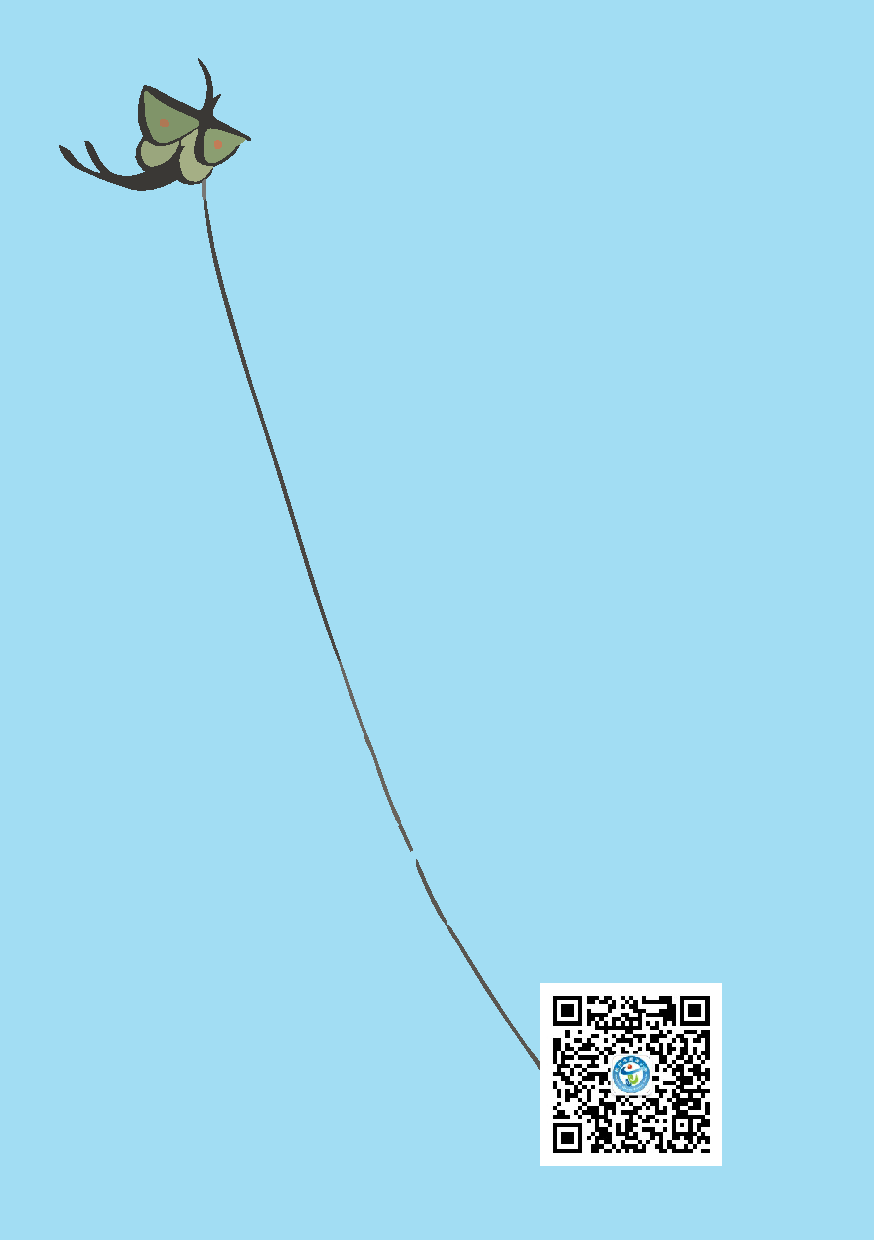
\includepdf{doc/hardback.pdf}
\end{document}
